\documentclass[oneside,final,14pt]{extreport}
\usepackage[utf8]{inputenc}
\usepackage[T2A,T1]{fontenc}
\usepackage[russian]{babel}
\usepackage{vmargin}
\usepackage{caption}
\usepackage{indentfirst}
\usepackage{setspace}
\usepackage{graphicx}
\usepackage{titlesec}
\usepackage{amsmath}
\usepackage{xinttools}
\usepackage{ragged2e}
\usepackage{ulem}
\usepackage{listings}
\usepackage{amsfonts}
\usepackage{color}
\usepackage{xstring}
\usepackage[abspath]{currfile}
\usepackage[hidelinks,linktoc=all]{hyperref}

\setpapersize{A4}
\setmarginsrb{1.5cm}{1.5cm}{1cm}{1.5cm}{0pt}{0mm}{0pt}{13mm}
\sloppy

\definecolor{dkgreen}{rgb}{0,0.6,0}
\definecolor{gray}{rgb}{0.5,0.5,0.5}
\definecolor{mauve}{rgb}{0.58,0,0.82}

\lstset{frame=tb,
    language=C++,
    aboveskip=3mm,
    belowskip=3mm,
    showstringspaces=false,
    columns=flexible,
    basicstyle={\small\ttfamily},
    numbers=none,
    numberstyle=\tiny\color{gray},
    keywordstyle=\color{blue},
    commentstyle=\color{dkgreen},
    stringstyle=\color{mauve},
    breaklines=true,
    breakatwhitespace=true,
    tabsize=3
}

\newcommand{\runtimeFsep}{/}
\newcommand{\updateRuntimeFsep}{\IfSubStr{\currfileabsdir}{/}{}{\renewcommand{\runtimeFsep}{\backslash}}}

\updateRuntimeFsep

\makeatletter
\DeclareRobustCommand{\filename}[2][]{%
    \begingroup
    % \lstname seems to change hyphens into \textendash
    \def\textendash{-}%
    \filename@parse{#2}%
    \IfSubStr{\filename@base}{\runtimeFsep}{\filename@parse{\filename@base}}{}%
    \edef\filename@base{\detokenize\expandafter{\filename@base}}%
    #1{\filename@base.\filename@ext}%
    \endgroup
}
\makeatother

\makeatletter
\newcommand\inputcode[3][]{
    {\bfseries #1\filename{#2}}:
    \lstinputlisting[%
        #3,
    ]{#2}%
}
\makeatother

\titleformat{\chapter}[display]
{\normalfont\large\bfseries}{\chaptertitlename\ \thechapter}{20pt}{\Large}

\newcommand\tcchapter[1]{%
    \chapter*{#1}%
    \addcontentsline{toc}{chapter}{#1}
}

\onehalfspacing

% NormalTeXSyntaxON
\def\setcase#1 {\expandafter\def\csname col:#1\endcsname}
\def\taskFileName#1{\expandafter\ifx\csname col:#1\endcsname\relax \coldefault 
                \else \csname col:#1\endcsname\fi}

\def\coldefault {code/taskN.cpp}    
\setcase 1      {code/task1.cpp} 
\setcase 2      {code/task2.cpp}
\setcase 3      {code/task3.cpp}

% NormalTeXSyntaxOff


\begin{document}
\lstset{language=[11]C++}

%title-page
\begin{titlepage}
    \begin{center}
        \begin{small}
            \begin{singlespace}
                \MakeUppercase{
                    МИНИСТЕРСТВО ОБРАЗОВАНИЯ И НАУКИ РФ\\ \vspace{0.7em}
                    Федеральное государственное бюджетное образовательное учреждение  высшего образования\\
                    ВЯТСКИЙ ГОСУДАРСТВЕННЫЙ УНИВЕРСИТЕТ\\ \vspace{0.7em}
                    Институт математики и информационных систем \\ \vspace{0.7em}
                    Факультет компьютерных и физико-математических наук\\ \vspace{0.7em}
                    Кафедра прикладной математики и информатики
                }
            \end{singlespace}
        \end{small}
        \vfill
        {\raggedleft
            Допущена к защите

            Заведующей кафедрой ПМИ

            \uline{\hspace{9em}}~Е.В.Разова

        }
        \vspace{5em}

        \MakeUppercase{
            \large{
                {\bfseries Приложения комплексных чисел к решению геометрических задач}
            }}
        \vspace{2em}

        Курсовой проект по дисциплине <<Проектная и научно-исследовательская деятельность>>
    \end{center}
    \vfill
    Выполнил студент группы ПМИб-2301-52-00 { \uline{\hspace{9em}}~/Г.Е. Ступников/}
    Руководитель к.ф-м.н. доцент кафедры ПМИ { \uline{\hspace{8.5em}}~/И.А. Пушкарев/
    }
    \vspace{2em}

    {\raggedright
        Работа защищена с оценкой \uline{\hspace{6em}} \hfill \uline{\hspace{2.5em}}.\uline{\hspace{2.5em}}.\the\year\
    }
    \vfill

    \begin{center}
        \MakeUppercase{Киров} \the\year\ г.
    \end{center}
\end{titlepage}
\setcounter{page}{2}

\thispagestyle{empty}
\clearpage

\tableofcontents

\tcchapter{Введение}
В настоящее время в большом количестве прикладных и научных областей возникает необходимость решения
геометрических задач. Основные из них - производство различных деталей и конструкций, моделирование
различных объектов и явлений. В данных областях возникает потребность поиска эффективного решения
поставленных задач, что подразумевает выборку оптимального метода решения или соотношения между ними.
Основные методы решения задач следующие\cite{geom:methods}:
\begin{enumerate}
   \item Аналитический. Состоит в представлении входных и требуемых данных в виде набора переменных и
         констант и взаимосвязи между ними в виде алгебраических уравнений с последующим их решением.
         \label{gmethod:enum1}
   \item Графический. Состоит в построении рисунка, полноценно отражающего набор необходимых для
         решения задачи входных данных и взаимосвязей между ними. Решение состоит в последовательном
         применении известных фактов и теорем, приводящих к получению ответа.
   \item Комбинация двух предыдущих. При ручном решении применяется чаще всего.
\end{enumerate}
Метод комплексных чисел является расширением аналитического метода~(метод~№\ref{gmethod:enum1}).
Он позволяет представить геометрические объекты 2-мерной плоскости в виде набора комплексных
чисел и равенств, отражающих взаимосвязи между ними.\\
Данный метод достаточно контринтуитивен и сложен для самостоятельного изучения (особенно
непривычно выглядит спиральное подобие как геом. ипостась умножения),при этом он не рассматривается
в школах на уровне основной программы \cite{edu:problem},\cite[стр.6]{book:ponarin}.\\
Проблема состоит в том, что для данного метода отсутствуют материалы для внедрения в среду
самостоятельного и школьного обучения, включающие программы, облегчающие изучение метода.\\
% 1. Метод контринтуитивен и непривычен для учащихся (подготовить мат. для внедрения)
% 2. Особенно непривычно выглядит спиральное подобие как геом. ипостась умножения
Целью данной работы является изучение метода комплексных чисел при решении геометрических задач,
реализация программной верификации решения выбранных задач.\\
Для достижения цели необходимо выполнить следующие задачи:
\begin{enumerate}
   \item Изучить имеющиеся способы применения алгебры комплексных чисел при решении геометрических
         задач.
   \item Выбрать задачи, на которых будет рассматриваться практическое применение метода.
   \item Решение задач с применением метода комплексных чисел
   \item Реализация программной верификации решения задач с применением метода.
\end{enumerate}

\tcchapter{Основные обозначения}
Комплексное число \(z\) -- число вида $x + iy$, где $x,y \in \mathbf{R}, i = \sqrt{-1},z \in \mathbf{C},
   \mathbf{C}$ - поле комплексных чисел. У числа \(z\) можно выделить действительную $x = Re(z)$ и
мнимую $y=Im(z)$ части \cite[стр. 357]{book:semendyaev}.

На плоскости зададим прямоугольную декартову систему координат \(Oxy\) и отображение $f: M(x;y)
   \leftrightarrow z = x + iy$, где $M \in \mathbf{P}$ -- точка плоскости с координатами $x,y \in
   \mathbf{R}, \mathbf{P}$ -- множество точек евклидовой плоскости. Комплексное число $z$ называют
комплексной координатой соответствующей точки $M$ и пишут \(M(z)\).
Отображение \(f\) биективно. Метод комплексных чисел основан на данном факте. Таким образом,
свойства и операции комплексных чисел можно перенести на прямоугольную декартову систему
координат евклидовой плоскости.

Для примера рассмотрим некоторые из свойств:
\begin{enumerate}
   \item Модуль числа $z = \vert z\vert = \sqrt{x_0^2+y_0^2} = r$ -- расстояние между точкой
         \(O\) и \(M\) (рис. \ref{theory-1}).
   \item Если $\angle \varphi$ -- ориентированный, образованный $\overrightarrow{OM}$
         с осью \(Ox\), то $x_0 = r\cos \varphi,~y_0 = r\sin \varphi$ (из определения функций).
         Тогда $z_0 = r(\cos \varphi + i \sin \varphi)$. Такое представление комплексного
         числа называют тригонометрическим.
   \item arg $z$ = $\angle \varphi$.
   \item Если существует вектор \(\overrightarrow{OM}\) (точка \(O\) -- начало координат),
         то отображение \(M(z) \rightarrow OM\) биективно \cite[стр. 32]{book:jaglom}.
   \item Из свойств операций над векторами следует, что сумме и разности векторов однозначно
         соответствуют сумма и разность соответствующих им комплексных чисел.
         \label{theory-properties}
\end{enumerate}
%TODO добавить признаки коллинеарности, дописать свойства
\begin{figure}[ht]
   \centering
   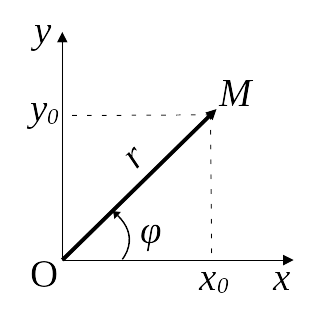
\includegraphics[width=0.33\textwidth]{images/theory-1}
   \caption{Изображение числа \(z\) на плоскости}
   \label{theory-1}
\end{figure}

\tcchapter{Решение и разбор задач с применением метода}
{
   \section*{Задача 1}
   \paragraph{Постановка задачи:}
   Точка \(D\) симметрична центру описанной около треугольника ABC окружности, относительно прямой AB.
   Доказать, что расстояние CD выражается формулой
   \begin{equation}
      CD^2 = R^2 +AC^2 + BC^2 - AB^2
      \label{t1:f1}
   \end{equation}
   где R - радиус описанной окружности.
   \begin{figure}[h]
      \centering
      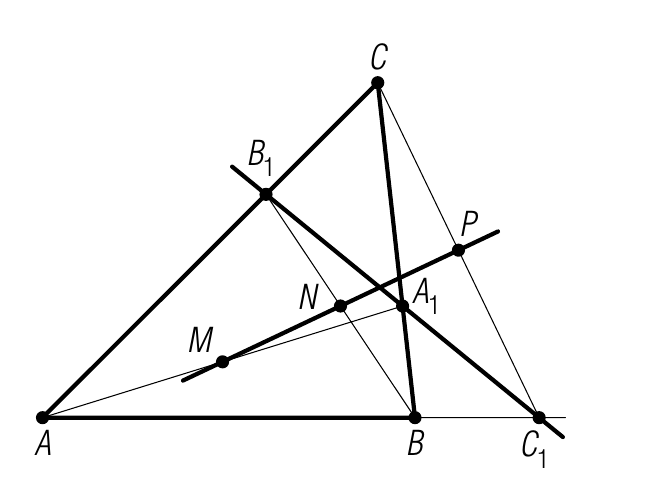
\includegraphics[width=0.5\textwidth]{images/task1.png}
      \caption{Иллюстрация к задаче}
      \label{t1:im}
   \end{figure}
   \paragraph{Решение задачи:}
   За начало координат плоскости будем считать точку \(O\) -- центр описанной около треугольника \(ABC\)
   окружности. Уравнение данной окружности имеет вид \(z\bar{z} = |z|^2 = x^2 + y^2 = R^2\), где
   \(z \in \mathbf{C}\). %TODO insert reference to rule
   Рассмотрим четырехугольник \(OADB\): \(OA = AD = OB = BD\)
   по условию задачи и отрезки \(AB, OD\) пересекаются под
   прямым углом, следовательно, \(OADB\) -- ромб. На основании
   данного факта верно следующее утверждение -- \(d = a + b\).
   Тогда
   \begin{equation}
      CD^2 =(d - c)(\bar{d} - \bar{c}) = (a + b - c)(\bar{a} +
      \bar{b} - \bar{c}) = 3R^2 + (a\bar{b} + \bar{a}b) - (a\bar{c} +
      \bar{a}c) - (b\bar{c} + \bar{b}c).
   \end{equation}
   Этому же выражению равна правая часть доказываемого
   равенства:
   \begin{equation}
      {
         \begin{aligned}
             & R^2 + AC^2 + BC^2 - AB^2 = R^2 + (a - c)(\bar{a} - \bar{c}) +
            (b - c)(\bar{b} - \bar{c}) - (a - b)(\bar{a} - \bar{b}) =        \\
             & = 3R^2 - (a\bar{c} + \bar{a}c) - (b\bar{c} + \bar{b}c) +
            (a\bar{b} + \bar{a}b)                                            \\
         \end{aligned}
      }
   \end{equation}
   Таким образом утверждение \ref{t1:f1} верно, что и требовалось доказать.

   \paragraph{Вычислительная иллюстрация на частном случае:}
   На вход программы передаются координаты свободных точек комплексной плоскости, в данном примере это
   координаты точек \(A,B,C\). Если \(A,B,C\) не лежат на одной прямой, то по данным входным данным
   строится описанная окружность и точки \(O, D\). Если условие \ref{t1:f1} выполняется, то задача
   считается решенной для данных входных данных и на экран выводятся координаты точек \(O, D\), а также
   координаты всех остальных. Блок-схема алгоритма приведена на Рис. \ref{t1:scheme}.
   \begin{center}
      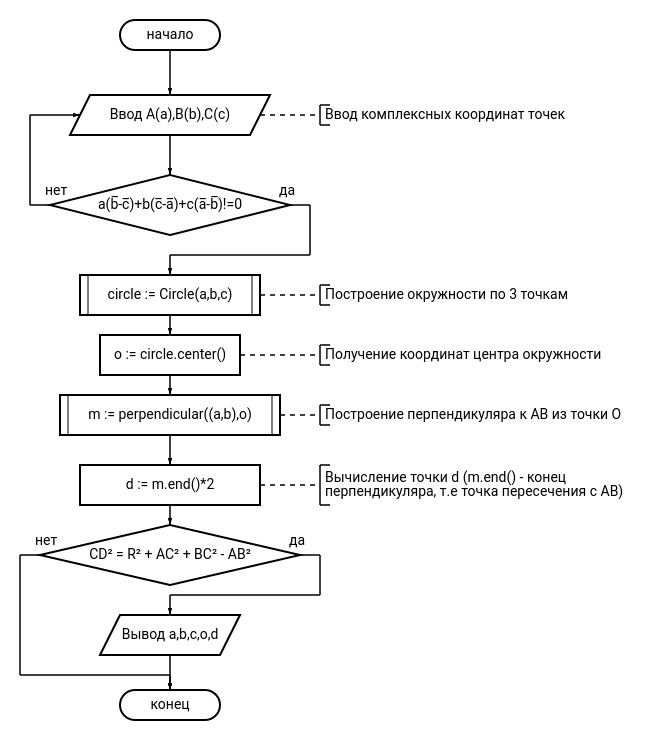
\includegraphics[width=0.9\textwidth]{images/task1-diagram.png}
      \captionof{figure}{Блок-схема алгоритма программы}
      \label{t1:scheme}
   \end{center}
   \paragraph{Программная реализация задачи:}
   Решение задачи написано на языке C++ в виде части программы для решения задач из данной работы.
   Реализация алгоритма программы предоставлена в функции task1::solve (файл \filename{\taskFileName{1}}):
   \lstinputlisting[frame=none,caption={Функция task1::solve},label=task1-code,captionpos=b,firstline=14]{\taskFileName{1}}
   \paragraph{Демонстрация работы:}
   TODO % TODO
}
{
   \section*{Задача 2}
   \paragraph{Постановка задачи:}
   Точка \(M\) -- середина дуги \(AB\) окружности. Доказать, что для произвольной точки N этой
   окружности имеет место
   равенство
   \begin{equation}
      \left\lvert AM^2-MN^2 \right\rvert = AN \cdot BN.
      \label{t2:f1}
   \end{equation}
   \paragraph{Решение задачи:}
   Пусть точкам \(A,B,M,N\) соответствуют комплексные числа \(a,b,m,n\). Для упрощения доказательства
   возьмем дугу \(AB\) такую, что \(a = \bar{b},b = \bar{a}\) и \(m = 1 + i0 = 1\) соответственно, и
   окружность радиуса \(r = 1\). За начало координат примем центр окружности (см рис. \ref{t2:im}).
   \begin{figure}[h]
      \centering
      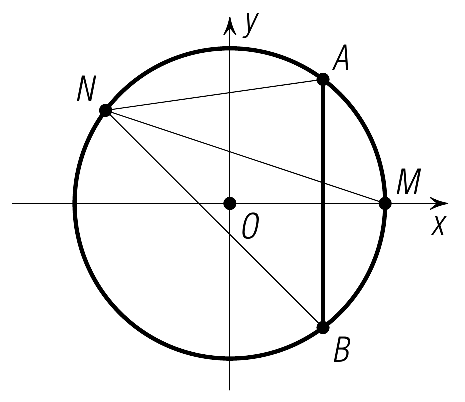
\includegraphics[width=0.5\textwidth]{images/task2.png}
      \caption{Иллюстрация к доказательству}
      \label{t2:im}
   \end{figure}
   Тогда уравнение окружности имеет
   вид \(z \bar{z}=1\), и поэтому \(a=\bar{b}, b=\bar{a}\).

   Находим:
   \(AN \cdot BN = \left\lvert a-n \right\rvert \cdot \left\lvert b-n \right\rvert
   = \left\lvert (a-n)(\bar{a}-n)\right\rvert
   = \left\lvert a\bar{a} - na - n\bar{a} + n^2 \right\rvert
   = \left\lvert 1 + n^2 - n(a+\bar{a})\right\rvert.\)

   Так как \(AM^2 =(a-1)(\bar{a}-1)\) и \(MN^2 =(n-1)(\bar{n}-1)\), то
   \(\left\lvert AM^2 - MN^2 \right\rvert = \left\lvert n+\bar{n}-(a+\bar{a}) \right\rvert\).
   Умножив это равенство на \(\left\lvert n \right\rvert=1\), получим:
   \(\left\lvert AM^2 - MN^2 \right\rvert = \left\lvert n^2 +1-n(a+\bar{a})\right\rvert = AN \cdot BN\).
   \paragraph{Вычислительная иллюстрация на частном случае:}
   Строится окружность радиуса \(r = 1\). На вход программы передаются координаты свободных точек комплексной
   плоскости, в данном примере это координаты точек \(A,B,N\),
   а также вспомогательная точка \(T\) (\(T \in AB\)), которая нужна для однозначного построения дуги. Если \(A,B,N\)
   принадлежат построенной окружности, то по данным
   входным данным вычисляются координаты точки \(M\). Если условие задачи (\ref{t2:f1}) выполняется, то задача
   считается решенной для данных входных данных и на экран
   выводятся координаты точки \(M\), а также координаты всех остальных. Блок-схема алгоритма приведена на
   Рис. \ref{t2:scheme}.
   \begin{center}
      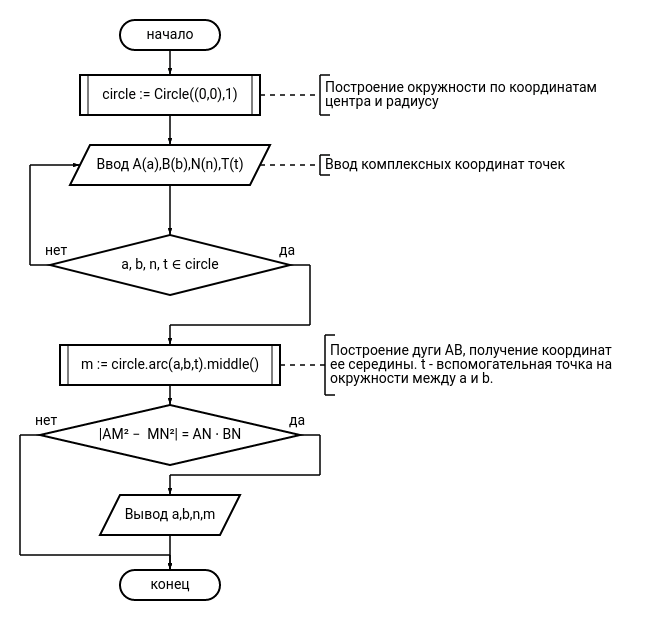
\includegraphics[width=0.9\textwidth]{images/task2-diagram.png}
      \captionof{figure}{Блок-схема алгоритма программы}
      \label{t2:scheme}
   \end{center}
   \paragraph{Программная реализация задачи:}
   Решение задачи написано на языке C++ в виде части программы для решения задач из данной работы.
   Реализация алгоритма программы предоставлена в функции task2::solve (файл \filename{\taskFileName{2}}):
   \lstinputlisting[frame=none,caption={Функция task2::solve},label=task2-code,captionpos=b,firstline=8]{\taskFileName{2}}
   \paragraph{Демонстрация работы:}
   TODO % TODO
}
{
   \section*{Задача 3}
   \paragraph{Постановка задачи:}
   Докажите, что сумма квадратов диагоналей параллелограмма
   равна сумме квадратов всех его сторон (Рис. \ref{t3:im}).
   Таким образом, требуется доказать, что
   \begin{equation}
      AD^2 + BC^2 = AB^2 +CD^2 + BD^2 + AC^2
      \label{t3:f1}
   \end{equation}
   \begin{figure}[h]
      \centering
      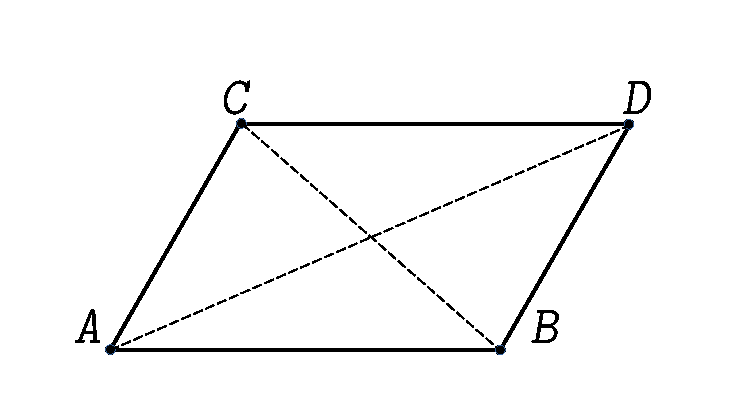
\includegraphics[width=0.7\textwidth]{images/task3.pdf}
      \caption{Иллюстрация к задаче}
      \label{t3:im}
   \end{figure}
   \paragraph{Решение задачи:}
   Зададим точку \(A(a) = 0 + i \cdot 0\).
   Тогда верны следующие утверждения: \(d = c + b\), \(\overrightarrow{CB} = b - c\).
   \begin{flalign}
      \label{t3:f2}
       & AB^2 + BD^2 + CD^2 + AC^2 = \left\lvert b\right\rvert^2 + \left\lvert c\right\rvert^2 + \left\lvert b\right\rvert^2 + \left\lvert c\right\rvert^2 = 2b\bar{b} + 2c\bar{c} &
   \end{flalign}
   \begin{flalign}
      \label{t3:f3}
       & AD^2 + BC^2 = \left\lvert d\right\rvert^2 + \left\lvert b - c\right\rvert^2 = d\bar{d} + (b-c)(\bar{b}-\bar{c}) = (c+b)(\bar{c}+\bar{c}) + b\bar{b} - b\bar{c} - & \\ \nonumber
       & - c\bar{b} + c\bar{c} = c\bar{c} + c\bar{b} + b\bar{c} + 2b\bar{b} + c\bar{c} - b\bar{c} - c\bar{b} = 2b\bar{b} + 2c\bar{c}                                      &
   \end{flalign}
   \noindent
   Таким образом, выражения (\ref{t3:f2}) и (\ref{t3:f3}) равны друг другу, что и требовалось доказать.

   \paragraph{Вычислительная иллюстрация на частном случае:}
   На вход программы передаются координаты свободных точек комплексной плоскости, в данном примере это координаты
   точек \(A,B,C\). Если \(A,B,C\) образуют треугольник, то по данным входным строится параллелограмм. Если
   условие задачи (\ref{t3:f1}) выполняется, то задача считается решенной для данных входных данных и на экран
   выводятся координаты точки \(D\), а также координаты всех остальных. Блок-схема алгоритма приведена
   на Рис. \ref{t3:scheme}.
   \begin{center}
      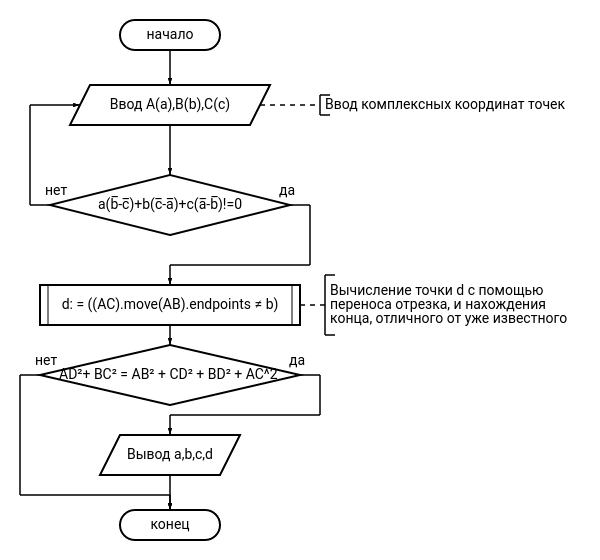
\includegraphics[width=0.9\textwidth]{images/task3-diagram.png}
      \captionof{figure}{Блок-схема алгоритма программы}
      \label{t3:scheme}
   \end{center}
   \paragraph{Программная реализация задачи:}
   Решение задачи написано на языке C++ в виде части программы для решения задач из данной работы.
   Реализация алгоритма программы предоставлена в функции task3::solve (файл \filename{\taskFileName{3}}):
   \lstinputlisting[frame=none,caption={Функция task3::solve},label=task3-code,captionpos=b,firstline=5]{\taskFileName{3}}
   \paragraph{Демонстрация работы:}
   TODO % TODO
}
{
   \section*{Задача 4}
   \paragraph{Постановка задачи:}
   Доказать, что если некоторая прямая пересекает прямые, содержащие стороны
   \(BC\), \(CA\), \(AB\) треугольника \(ABC\), в точках \(A_1\) , \(B_1\) , \(C_1\)
   соответственно, то середины отрезков \(AA_1\) , \(BB_1\) , \(CC_1\) коллинеарны (Рис. \ref{t5:im}).
   \begin{figure}[h]
      \centering
      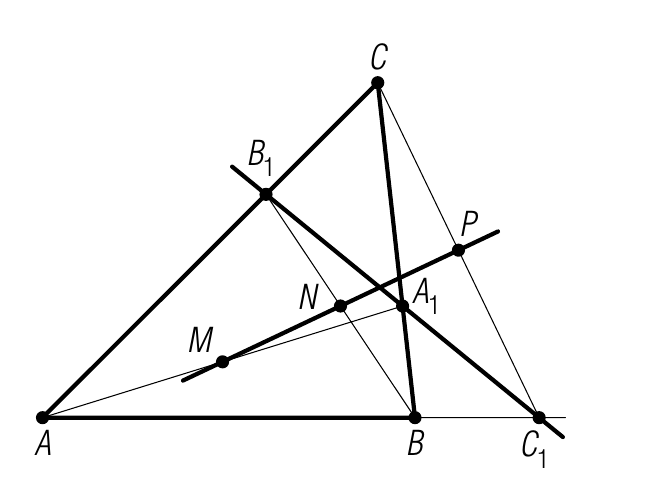
\includegraphics[width=0.5\textwidth]{images/task4.png}
      \caption{Иллюстрация к задаче}
      \label{t4:im}
   \end{figure}
   \paragraph{Решение задачи:}
   %FIXME Для решения данной задачи требуется найти достаточные критерии коллинеарности точек 3 точек.
   Условие коллинеарности троек точек \(A, B_1 , C\); \(C,
   A_1 , B\); \(B, C_1 , A\); \(A_1 , B_1 , C_1\):

   \begin{equation}
      \left\{ \begin{aligned}
          & a(\bar{b_1} - \bar{c}) + b_1(\bar{c} - \bar{a}) + c(\bar{a} - \bar{b_1}) = 0             \\
          & b(\bar{c_1} - \bar{a}) + c_1(\bar{a} - \bar{b}) + a(\bar{b} - \bar{c_1}) = 0             \\
          & c(\bar{a_1} - \bar{b}) + a_1(\bar{b} - \bar{c}) + b(\bar{c} - \bar{a_1}) = 0             \\
          & a_1(\bar{b_1} - \bar{a_1}) + b_1(\bar{a_1} - \bar{a_1}) + a_1(\bar{a_1} - \bar{b_1}) = 0 \\
      \end{aligned}
      \right. \label{t4:f1}
   \end{equation}
   Если \(M, N, P\) -- середины отрезков \(AA_1, BB_1, CC_1\), то предстоит показать, что
   \begin{equation}
      m(\bar{n} -\bar{p})+n(\bar{p}-\bar{m})+p(\bar{m}-\bar{n})=0,
      \label{t4:f2}
   \end{equation}
   Так как \(\displaystyle
   m=\frac{1}{2}(a+a_1),\;
   n=\frac{1}{2}(b+b_1),\;
   p=\frac{1}{2}(c+c_1)
   \), то доказываемое равенство (\ref{t4:f2}) эквивалентно такому:

   \(
   (a+a_1)(\bar{b}+\bar{b_1}-\bar{c}-\bar{c_1})+(b+b_1 )(\bar{c}+\bar{c_1}-\bar{a}-\bar{a_1})+(c+c_1)(\bar{a}+\bar{a_1}-\bar{b}-\bar{b_1})=0,
   \) или, после перемножения,
   \begin{equation}
      \begin{aligned}
          & a(\bar{b_1} - \bar{c}) + a(\bar{b}- \bar{c_1}) + a_1(\bar{b_1} - \bar{c_1}) + a_1(\bar{b}- \bar{c}) + b(\bar{c_1} - \bar{a}) + b(\bar{c}- \bar{a_1}) + \\
          & +b_1(\bar{c_1}-\bar{a_1})+b_1 (\bar{c}-\bar{a})+c(\bar{a_1}-\bar{b})+c(\bar{a}-\bar{b_1})+c_1 (\bar{a_1}-\bar{b_1} )+c_1(\bar{a}-\bar{b})=0.
      \end{aligned}
      \label{t4:f3}
   \end{equation}
   Теперь легко видеть, что (\ref{t4:f3}) получается при почленном сложении
   равенств (\ref{t4:f1})
   \paragraph{Вычислительная иллюстрация на частном случае:} На вход программы передаются координаты
   свободных точек комплексной плоскости, в данном примере это координаты точек \(A,B,C,A_1,B_1\). Если \(A_1,B_1\)
   лежат на треугольнике, то по данным входным данным строится прямая, соответствующая условиям задачи. Далее
   производится проверка того, что середины отрезков \(AA_1,BB_1,CC_1\) коллинеарны. Если условие выполняется, то задача
   считается решенной для данных входных данных и на экран выводятся координаты точек \(M,N,P\), а также координаты
   всех остальных. Блок-схема алгоритма приведена на Рис. \ref{t4:scheme}.
   \begin{center}
      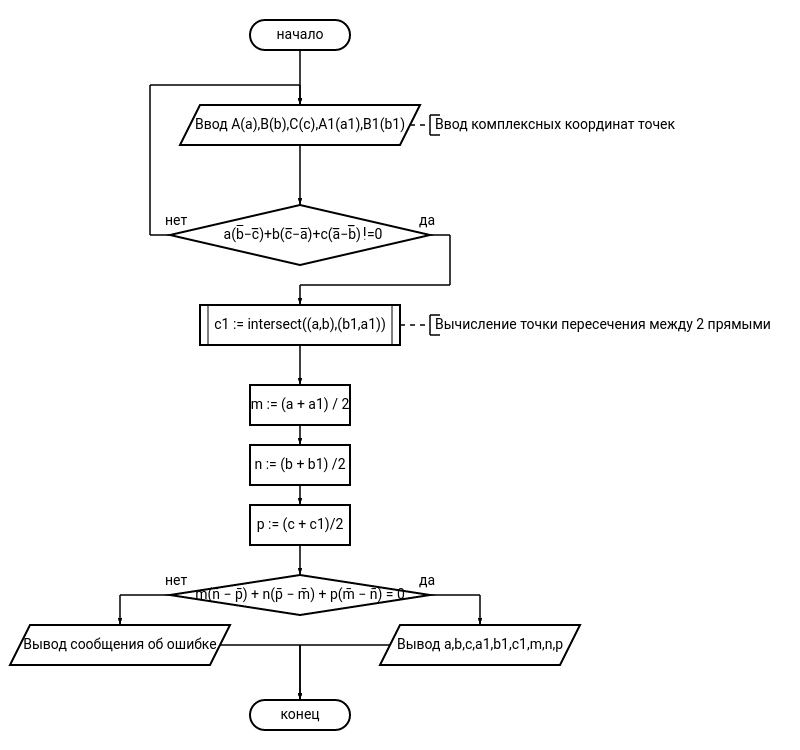
\includegraphics[width=0.79\textwidth]{images/task4-diagram.png}
      \captionof{figure}{Блок-схема алгоритма программы}
      \label{t4:scheme}
   \end{center}

   \paragraph{Программная реализация задачи:} Решение задачи написано на языке C++ в виде части
   программы для решения задач из данной работы.
   Реализация алгоритма программы предоставлена в функции task4::solve (файл \filename{\taskFileName{4}}):
   \lstinputlisting[frame=none,caption={Функция task4::solve},label=task4-code,captionpos=b,firstline=5]{\taskFileName{4}}
   \paragraph{Демонстрация работы:}
   Здесь будут скриншоты работы. TODO % TODO
}
{
   \section*{Задача 5}
   \paragraph{Постановка задачи:}
   Докажите, что диагонали вписанного в окружность четырёхугольника перпендикулярны, тогда и только тогда,
   когда сумма квадратов его противоположных сторон равна квадрату диаметра описанной окружности (Рис.~\ref{t5:im}).
   Таким образом, требуется доказать, что
   \begin{equation}
      AB^2+CD^2 = AC^2+BD^2 = PB^2 \Rightarrow AD \perp CB
      \label{t5:f1}
   \end{equation}
   \begin{figure}[h]
      \centering
      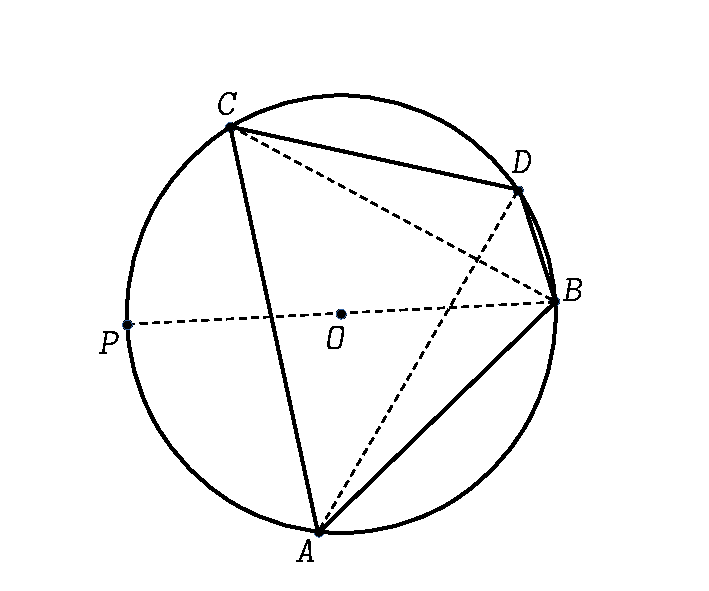
\includegraphics[width=0.7\textwidth]{images/task5.pdf}
      \caption{Иллюстрация к задаче}
      \label{t5:im}
   \end{figure}
   \paragraph{Решение задачи:}
   Обозначим диаметр окружности как \(PB\); будем считать, что окружность единичная с центром в т.\(O\).

   Исходя из свойств комплексных чисел, верно следующее:
   \begin{equation*}
      AD \perp CB \Leftrightarrow (d-a)(\bar{b}-\bar{c})+(\bar{d}-\bar{a})(b-c) = 0
      \label{t5:f2}
   \end{equation*}

   Из условий задачи:
   \begin{equation}
      \left\{ \begin{aligned}
          & (a - b)(\bar{a} - \bar{b}) + (c - d)(\bar{c} - \bar{d}) = (p - b)(\bar{p} - \bar{b}) \\
          & (a - c)(\bar{a} - \bar{c}) + (b - d)(\bar{b} - \bar{d}) = (p - b)(\bar{p} - \bar{b}) \\
      \end{aligned}
      \right. \label{t5:f3}
   \end{equation}

   Почленно вычтя второе уравнение системы (\ref{t5:f3}) из первого, получаем:
   \begin{flalign*}
      \label{t5:f4}
       & a\bar{a} - a\bar{b} - b\bar{a} + b\bar{b} + c\bar{c} - c\bar{d} - d\bar{c} + d\bar{d} - a\bar{a} + a\bar{c} + c\bar{a} - c\bar{c} - b\bar{b} + b\bar{d} + & \\ \nonumber
       & + d\bar{b} - d\bar{d} = 0 \Leftrightarrow - a\bar{b} - b\bar{a} - c\bar{d} - d\bar{c} + a\bar{c} + c\bar{a} + b\bar{d} + d\bar{b} = 0 \Leftrightarrow     & \\ \nonumber
       & (d-a)(\bar{b}-\bar{c})+(\bar{d}-\bar{a})(b-c) = 0 \Leftrightarrow AD \perp CB                                                                             &
   \end{flalign*}
   Таким образом, утверждение (\ref{t5:f1}) доказано.
   \paragraph{Вычислительная иллюстрация на частном случае:} На вход программы передаются координаты
   свободных точек комплексной плоскости, в данном примере это координаты точек \(A,B,C,D\), по ним
   строится окружность. Если условие (\ref{t5:f1}) выполняется (вместо \(PB\) используется конструкция
   \(2OB\)), то задача считается решенной для данных входных данных и на экран выводятся
   координаты точки \(O\), а также координаты всех остальных. Блок-схема алгоритма приведена
   на Рис. \ref{t5:scheme}.
   \begin{center}
      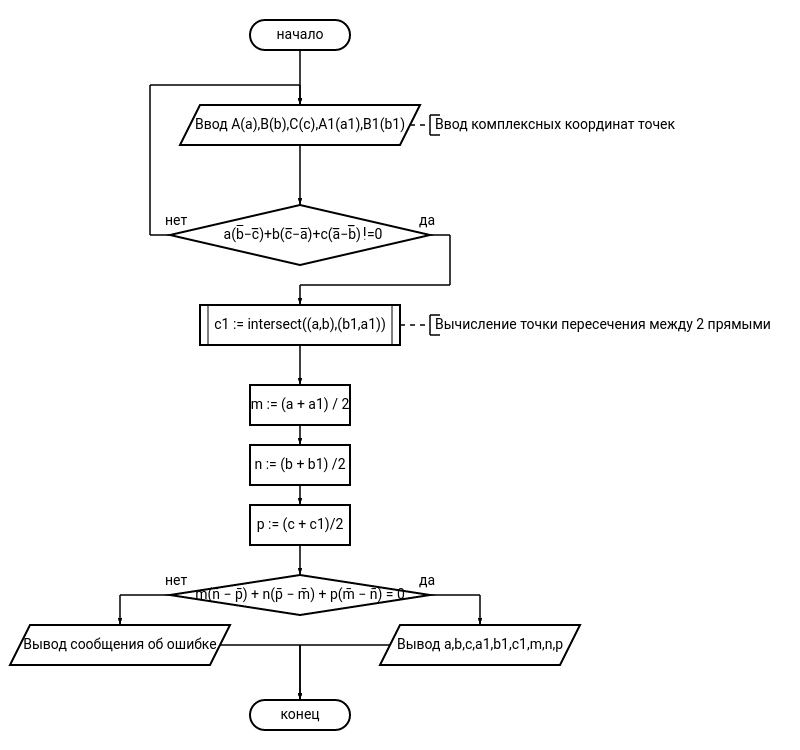
\includegraphics[width=0.79\textwidth]{images/task5-diagram.png}
      \captionof{figure}{Блок-схема алгоритма программы}
      \label{t5:scheme}
   \end{center}

   \paragraph{Программная реализация задачи:} Решение задачи написано на языке C++ в виде части
   программы для решения задач из данной работы.
   Реализация алгоритма программы предоставлена в функции task5::solve (файл \filename{\taskFileName{5}}):
   \lstinputlisting[frame=none,caption={Функция task5::solve},label=task5-code,captionpos=b,firstline=5]{\taskFileName{5}}
   \paragraph{Демонстрация работы:}
   TODO % TODO
}
{
   \section*{Задача 6}
   \paragraph{Постановка задачи:}
   Докажите, что если средние линии четырёхугольника равны,
   то его диагонали перпендикулярны, и обратно (Рис. \ref{t6:im}).
   \begin{figure}[h]
      \centering
      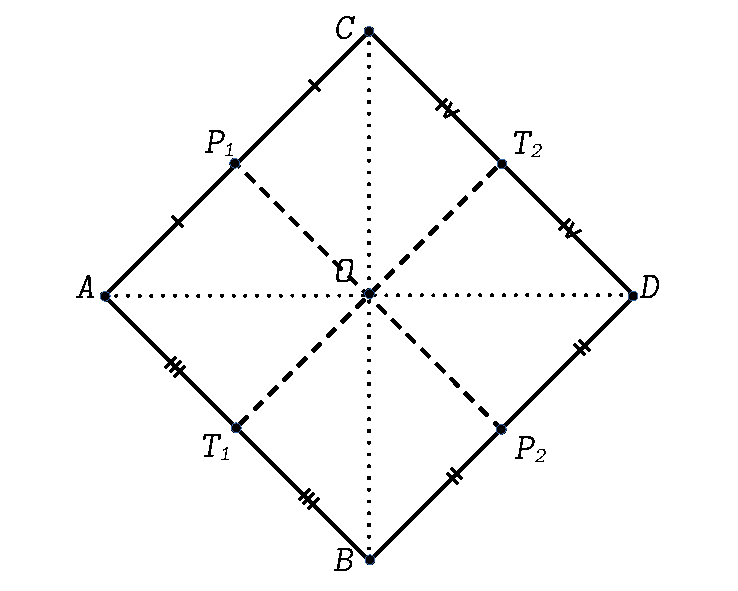
\includegraphics[width=0.5\textwidth]{images/task6.pdf}
      \caption{Иллюстрация к задаче}
      \label{t6:im}
   \end{figure}
   \paragraph{Решение задачи:}
   Точка \(O\) -- точка пересечения диагоналей четырёхугольника.
   Концы средних линий четырёхугольника имеют следующие координаты:
   \begin{equation}
      \frac{1}{2}(c+d),\frac{1}{2}(a+b),\frac{1}{2}(a+c),\frac{1}{2}(b+d).
      \label{t6:f1}
   \end{equation}
   Если средние линии четырёхугольника равны, то на основании (\ref{t6:f1}) и свойств комплексных чисел, при \(AD \neq 0, CB \neq 0\), получаем следующее:
   \begin{flalign*}
       & \left\lvert \frac{1}{2}(c+d) - \frac{1}{2}(a+b)\right\rvert = \left\lvert \frac{1}{2}(a+c) - \frac{1}{2}(b+d)\right\rvert \Leftrightarrow  \left(\frac{1}{2}(c+d) - \frac{1}{2}(a+b)\right) \cdot                                & \\
       & \left(\frac{1}{2}(\bar{c}+\bar{d}) - \frac{1}{2}(\bar{a}+\bar{b})\right) = \left(\frac{1}{2}(a+c) - \frac{1}{2}(b+d)\right) \cdot \left(\frac{1}{2}(\bar{a}+\bar{c}) - \frac{1}{2}(\bar{b}+\bar{d})\right) \Leftrightarrow       & \\
       & \frac{1}{2}\left((c+d) - (a+b)\right) \cdot \frac{1}{2}\left((\bar{c}+\bar{d}) - (\bar{a}+\bar{b})\right) = \frac{1}{2}\left((a+c) - (b+d)\right) \cdot \frac{1}{2}\left((\bar{a}+\bar{c}) - \vphantom{(\bar{c}+\bar{d})}\right. &
   \end{flalign*}
   \begin{flalign*}
       & \left. (\bar{b}+\bar{d})\vphantom{(\bar{c}+\bar{d})}\right) \Leftrightarrow                                                                                                                     & \\
       & \left(c + d - a - b\right) \cdot \left(\bar{c}+\bar{d} - \bar{a} - \bar{b}\right) = \left(a + c - b - d\right) \cdot \left(\bar{a} + \bar{c} - \bar{b} - \bar{d}\right) \Leftrightarrow         & \\
       & a\bar{c} - a\bar{b} + c\bar{a} - c\bar{d} - b\bar{a} + b\bar{d} - d\bar{c} + d\bar{b} = - a\bar{c} + a\bar{b} - c\bar{a} + c\bar{d} + b\bar{a} - b\bar{d} + d\bar{c} - d\bar{b} \Leftrightarrow & \\
       & a\bar{c} - a\bar{b} + c\bar{a} - c\bar{d} - b\bar{a} + b\bar{d} - d\bar{c} + d\bar{b} = 0 \Leftrightarrow                                                                                       & \\
       & (a-d)(\bar{c} - \bar{b}) + (c-b)(\bar{a} - \bar{d})  = 0                                                                                                                                        &
   \end{flalign*}

   Тогда \(2 \overrightarrow{AD} \overrightarrow{CB} = 0\Leftrightarrow \left\lvert AD\right\rvert
   \left\lvert CB\right\rvert \cos{\angle{COD}} \Leftrightarrow \angle{COD} = 90^\circ\),
   что и требовалось доказать.

   Если диагонали четырёхугольника перпендикулярны, то \(\angle{COD} = 90^\circ \Leftrightarrow \left\lvert AD\right\rvert \left\lvert CB\right\rvert \cos{\angle{COD}} = 0 \Leftrightarrow \overrightarrow{AD}\overrightarrow{CB}=
   0 \dots\)
   Дальнейшие рассуждения выполняются в порядке, обратном доказательству в случае, когда средние линии четырёхугольника равны.

   Таким образом, если средние линии четырёхугольника равны, то его диагонали перпендикулярны и наоборот.
   \paragraph{Вычислительная иллюстрация на частном случае:} На вход программы передаются координаты
   свободных точек комплексной плоскости, в данном примере это координаты вершин четырёхугольника \(A,B,C,D\) (выпуклого).
   Если средние линии четырёхугольника равны и его диагонали перпендикулярны, то задача
   считается решенной для данных входных данных и на экран выводятся координаты концов средних линий четырёхугольника, а также координаты
   всех остальных точек. Блок-схема алгоритма приведена на Рис. \ref{t6:scheme}.
   \begin{center}
      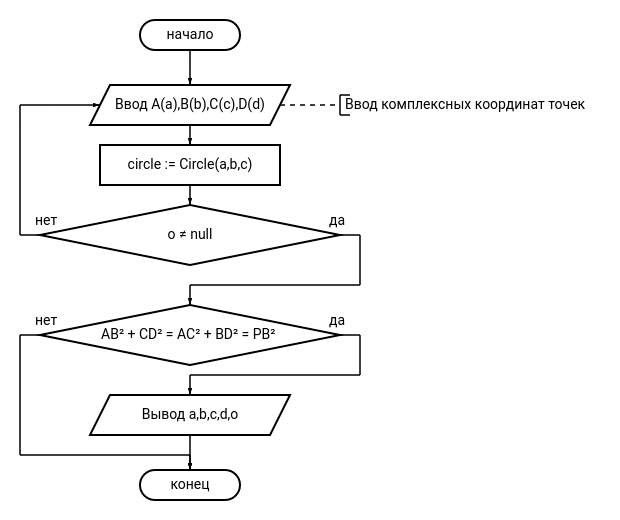
\includegraphics[width=0.9\textwidth]{images/task6-diagram.png}
      \captionof{figure}{Блок-схема алгоритма программы}
      \label{t6:scheme}
   \end{center}
   \paragraph{Программная реализация задачи:} Решение задачи написано на языке C++ в виде части
   программы для решения задач из данной работы.
   Реализация алгоритма программы предоставлена в функции task6::solve (файл \filename{\taskFileName{6}}):
   \lstinputlisting[frame=none,caption={Функция task6::solve},label=task6-code,captionpos=b,firstline=6]{\taskFileName{6}}
   \paragraph{Демонстрация работы:}
   TODO % TODO
}
\tcchapter{Заключение}
В ходе выполнения работы изложены основы метода комплексных чисел, было проиллюстрировано его
применение при решении 3 задач. Каждая задача имеет решение на языке C++.


Таким образом, все поставленные задачи были успешно выполнены, цель
достигнута.
%bibliography
\renewcommand\bibname{Список литературы}
\begin{thebibliography}{00}
   \addcontentsline{toc}{chapter}{Список литературы}
   \bibitem{book:ponarin} Понарин~Я.П. Алгебра комплексных чисел в геометрических задачах:
   Книга для учащихся математических классов школ, учителей и студентов педагогических вузов. --~М.:~МЦНМО,
   2004. -- 160 с.
   \bibitem{book:takeuti} Такеути Г. Теория доказательств. -- Пер. с англ. --~М.:~Мир, 1978. -- 414 с.
   \bibitem{book:sloyer} Слойер К. Математические фантазии. -- Пер. с англ. --~М.:~Мир, 1993. -- 184 с.
   \bibitem{book:kosnevsky} Коснёвски Ч. Занимательная математика и персональный компьютер. -- Пер. с англ. --~М.:~Мир, 1987. -- 192 c.
   \bibitem{geom:methods} Кибирев~В.~В. Обучение методам решения геометрических задач // Вестник~БГУ.~2014.~№15. URL:~\href{https://cyberleninka.ru/article/n/obuchenie-metodam-resheniya-geometricheskih-zadach}{https://cyberleninka.ru/article/n/obuchenie-metodam-resheniya-geometricheskih-zadach} (дата обращения:~19.07.2022).
   \bibitem{book:semendyaev} Бронштейн~И.~Н., Семендяев~К.~А. Справочник по математике для инженеров и учащихся втузов.-- 13-е изд., исправленное. --~М.:~Наука, Гл.~ред.~физ.-мат.~лит., 1986. -- 544 с.
   \bibitem{book:arnold_complex} Арнольд~В.~И.Геометрия комплексных чисел, кватернионов и спинов. -- 4-е изд., стереотипное. --~М.:~МЦНМО, 2014. -- 40 с.
   \bibitem{book:jaglom} Яглом~И.~М., Семендяев~К.~А. Комплексные числа и их применения в геометрии.-- 2-е изд., стереотипное. --~М.:~Едиториал~УРСС, 2004. -- 192 с.
   \bibitem{edu:problem} Жмурова~И.~Ю. Изучение комплексных чисел в общеобразовательной школе / И.~Ю.~Жмурова, С.~В.~Баринова. // Молодой~ученый. -- 2020. -- №~5~(295). -- С.~312-314. -- URL:~\href{https://moluch.ru/archive/295/67123/}{https://moluch.ru/archive/295/67123/} (дата обращения: 17.05.2022).
\end{thebibliography}

\clearpage
\tcchapter{Приложения}
\appendix
% FIXME TOC format of the sections
\titleformat{\section}[block]{\bfseries}{Приложение \Alph{section}.}{1em}{}[]
\renewcommand{\thesection}{\Alph{section}}

\section{Листинг программы}
{\setlength{\parindent}{0cm}
\inputcode[Файл меню ]{code/main.cpp}{frame=none}
\inputcode{\taskFileName{1}}{frame=none}
\inputcode{\taskFileName{2}}{frame=none}
\inputcode{\taskFileName{3}}{frame=none}
% TODO add more tasks
\vspace{20pt}

\inputcode{code/functions.hpp}{frame=none}
\inputcode{code/functions.cpp}{frame=none}

\vspace{20pt}
\inputcode{code/ComplexNumber.hpp}{frame=none}
\inputcode{code/ComplexNumber.cpp}{frame=none}

\vspace{20pt}
\inputcode{code/Line.hpp}{frame=none}
\inputcode{code/Line.cpp}{frame=none}

\vspace{20pt}
{\bfseries Определение класса Point (header-only):}\\
\inputcode{code/Point.hpp}{frame=none}
}


\end{document}
